\section{Connessione}
Un grafo si dice \textit{connesso} se - a partire da un nodo qualsiasi - posso raggiungerne un altro qualsiasi.
Qualora non sia connesso, si definisce \textit{componente connesso} qualsiasi sezione connessa che lo compone.

\section{Visitare un grafo}
Esistono due tipi di visita:
\begin{enumerate}
    \item Visita in profondità
    \item Visita in ampiezza
\end{enumerate}

\subsection{Visita in profondità}
Rappresenta una visita ricorsiva del grafo, partendo da un nodo generico scelto arbitrariamente. \\
Si costruisce un vettore binario \textit{v} (i cui valori sono inizialmente impostati tutti a \textit{0} - con costo $O(n)$), composto da n componenti, utilizzato per tenere traccia se il nodo preso in esame è già stato visitato (e quindi il suo valore sul vettore sarà impostato ad \textit{1}) o meno. \\
\begin{center}
    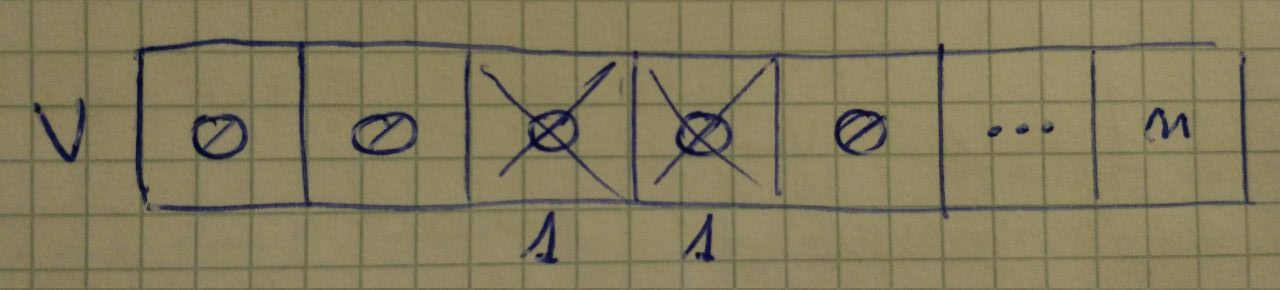
\includegraphics[width=.8\textwidth]{res/vettore-visita.jpg} \hfill
\end{center}
\newpage

L'algoritmo di \textit{visita in profondità} prende il nome di \textit{DFS}, che sta per \textit{Depth First Search}.
Inizializzato il vettore a \textit{0}, eseguo la procedura \textit{DFS(x)}:
\begin{lstlisting}
DFS(x)
    vis[x] <- 1         # imposto il valore del nodo ad 1
    for y in adj(x)     # itero sui nodi adiacenti ad x
        if vis[y]==0 then DFS(y)
\end{lstlisting}

Chiaramente, se al termine della visita \textit{v} contiene ancora alcuni \textit{0}, significa che il grafo non è connesso. \\
Genericamente la procedura \textit{DFS(x)} ha complessità di $O(n)$. Inoltre, però, questa fa un'iterazione (attraverso il ciclo \textit{for}) per ogni adiacenza col nodo, impiegando - nel caso peggiore - \textit{n} - caso in cui, quindi, il nodo abbia numero di adiacenze pari al numero totale di nodi. Di conseguenza, la procedura di visita impiega al più $O(n^2)$. \\
Se questa procedura - invece di lavorare con un vettore - lavora sulla rappresentazione a matrice, il caso peggiore che abbiamo analizzato, diventa l'unico caso possibile, per cui $\theta(n^2)$. \\
Infine, utilizzando la rappresentazione tramite liste di adiacenze, la procedura avrà complessità $O(n+m)$. \\\\
Tramite il percorso seguito dalle chiamate \textit{DFS(x)} è inoltre possibile ricavarci un albero, la cui radice è proprio la sorgente da cui si è partiti nella visita del grafo. \\
Inoltre, tramite lo stesso algoritmo - aggiungendo codice e/o funzioni - è possibile ottenere funzionalità particolari e aggiuntive, come la costruzione di un \textit{vettore dei padri}, un vettore che associa ad ogni nodo il corrispettivo padre nella rappresentazione dell'albero ottenuto tramite la visita del grafo.
\newpage

\begin{algorithm}
    \caption{Verifica di presenza di un ciclo}\label{alg:VPC}
    \begin{algorithmic}[1]
        \Function{HasCicli}{$x$}\Comment{Verifica la presenza di un ciclo}
            \State $ {vis}(x) \gets 1$ \Comment{Flag di visita}
            \For { $y \in {adj}(x)$} \Comment{Lista di adiacenza di x}
                \If ${ (a)= {true} }$
                    \Return true $(y)$ \Comment{Ricorsione per ricerca in profondità}
                \EndIf
            \EndFor
            \State \textbf{return} false\Comment{}
        \EndFunction
    \end{algorithmic}
\end{algorithm}

Secondo il professore l'algoritmo non è ottimizzato.
Prendiamo il vettore dei padri: l'unica cosa che avremmo dovuto fare per tenerlo aggiornato sarebbe stata P[n] <- e poi chiamiamo cicli(u), con questa istruzione ogni nodo saprebbe chi è il padre.

Analizziamo ora la complessità di questo algoritmo, e qui interviene il quesito secondo il quale ci chiediamo quale tipologia di implementazione del grafo dovremmo usare:
Ipotizzando di avere le liste di adiacenza: $O(n+m)$, che è la partenza del DFS(u), e vale $O(n)$. Supponiamo che il grafo sia aciclico, allora io dico che si ferma in $O(n)$, se è aciclico è un albero (in cui n = m). Se invece fosse ciclico: appena lo trovo mi fermo. Certamente creo un ciclo perché per non avere cicli possono esserci al più $n-1$, quindi non visita tutto il grafo, ma dopo al più $n-1$ si ferma: questo significa che dato un grafo, vedere se nel grafo c'è un ciclo, si può fare in $O(n)$ indipendentemente dagli archi che ho nel grafo. Ad essere precisi, se la applico non posso dire se il grafico è aciclico o meno, perché se fosse sconnesso se mi restituisce true vuol dire che c'è un ciclo che è collegato alla zona da cui comincio. Ma se risponde false, essendo sconnesso, potrebbe esserci un ciclo all'interno di una parte separata di grafo. Quindi in realtà questo algoritmo funziona solo in un grafo connesso. Per visitare anche pezzi diversi del grafo devo fare sostanzialmente più visite. \\

Se mi risponde false vado a scorrermi il vettore dei visitati, se tutto è stato visitato bene, ma se trovo un nodo che abbia valore 0 signfiica che si trova in una parte del grafo non raggiungibile, quindi vado a verificare quella parte del grafo, e se mi risponde false continuo a scorrere quello stesso vettore fino a quando il vettore è finito e tutti i nodi avranno valore 1. Non sto aumentando la complessità, perché mi costera $o(n(1))$, poi $o(n(2))$ + \ldots comunque sommati avrò in definitiva $O(n)$. Scritta in codice, la modifica risulta:

\begin{algorithm}
    \caption{VPC grafo non connesso}\label{alg:VPCnC}
    \begin{algorithmic}[1]
        \Function{HasCicliDisconnectedGraph}{$x$}\Comment{Verifica la presenza di un ciclo}
            \State ${vis}(x) \gets 1$ \Comment{Flag di visita}
            \For {$ i= 1 \rightarrow n$} \Comment{}
                \If {$ {vis}(i)= 0 {} $} $c \gets {ciclo}(i) $
                \EndIf
                \If {$ {}(b)= {true} $}
                    \Return true $(y)$ \Comment{}
                \EndIf
            \EndFor
            \State \textbf{return} false\Comment{}
        \EndFunction
    \end{algorithmic}
\end{algorithm}

Mentre nella visita di un grafo indiretto gli archi dell'albero risultante sono bipartiti, in quella di un grafo diretto gli archi sono \textit{quadripartiti}:
\begin{itemize}
	\item \textit{arco albero}: arco standard di un albero
	\item \textit{arco di attraversamento} o cross: arco laterale che va da destra a sinistra
	\item \textit{arco in avanti}: da antenato a discendente
	\item \textit{arco all'indietro} o back: da discendente ad antenato
\end{itemize} 
Per distinguere gli archi fwd/cross da back, si sottolinea la proprietà che i nodi che formano archi back non hanno finito la ricorsione in DFS.
Per sottolineare questa differenza, si inserisce nella funzione DFS l'istruzione che associa ad un nodo - nel vettore V - il valore 2 una volta finita la ricorsione (fuori dal for loop).\\
Per distinguere invece gli archi in avanti dai cross, occorre introdurre un nuovo vettore T che associ ogni nodo ad un valore numerico che ne indica l'ordine di visita: in questo modo sappiamo che i cross uniscono un nodo con un numero più grande (quindi visitato dopo) ad un nodo con un numero minore (viceversa per gli archi in avanti).
\paragraph{Esercizio}
Numerare ogni tipo di arco dell'albero derivato dalla visita partita dal nodo \textit{u}.\\
\begin{lstlisting}
tree = 0
back = 0
forw = 0
cros = 0
time = 0
V = [0|0|0|0|0|0|0|0|0|0|0|0|0|0|--]
T = [0|0|0|0|0|0|0|0|0|0|0|0|0|0|--]
DFS(x)
	vis[x] = 1 
	time++
	T[x] = time
	for y in adj(x)
		albero++
		if vis[y]==0
			then DFS(y)
		else
			if vis[y] == 1
				then back++
			else if t[x] < t[y]
				forw++
			else
				cross++
	vis[x] = 2
\end{lstlisting}
\newpage

\subsection{Visita in Ampiezza}
Dato un grafo, partendo da un nodo arbitrario, visito prima tutti i nodi ad esso adiacenti (nodi \textit{a distanza 1}). Poi, una volta visitati tutti, per ciascuno, visito i suoi adiacenti \textit{non visitati}. \\
L'albero formato da una visita in ampiezza è detto \textit{albero dei cammini minimi}, in quanto rappresenta il cammino più breve che intercorre tra la radice e un nodo qualsiasi del grafo. \\
L'algoritmo di \textit{visita in ampiezza} prende il nome di \textit{BFS}, che sta per \textit{Breadth First Search}.
\begin{lstlisting}
BFS(u)
	vis[u] = 1
    inizializza la coda Coda inserendo u
    while Coda != 0 do
        x = estrai dalla coda
        for y in adj(x) do
            if vis[y] = 0 then
                vis[y] = 1
                metti y in Coda
\end{lstlisting}
Analogamente, per costruire il vettore dei Padri, basta sostituire le occorrenze di \textit{vis} con il vettore \textit{Padri}. Utilizzando questa versione, costruiamo l'algoritmo per la costruzione delle distanza nodo-radice:
\begin{lstlisting}
# si inizializza il vettore Distanze a +infinito
BFS(u)
    Padri[u] = 0
    Distanza[u] = 0
    inizializza la coda Coda inserendo u
    while Coda != 0 do
        x = estrai dalla coda
        for y in adj(x) do
            if Padri[y] = 0 then
                Distanza[y] = Distanza[x] + 1
                Padri[y] = x
                metti y in Coda
\end{lstlisting}
\subsubsection{Dimostrazione correttezza algoritmo per induzione}
$\forall k \geq 0$ $\exists$ un'istante di tempo in cui:
\begin{enumerate}
    \item tutti i nodi con distanza $\leq k$ avranno il loro valore correttamente calcolato nel vettore Distanza;
    \item in quel momento, in coda ci sono solo i nodi a distanza \textit{k}.
\end{enumerate}
\paragraph{PASSO BASE.}
$k=0$ definisce il caso della radice, per il quale abbiamo in coda solo la radice.
\paragraph{PASSO INDUTTIVO}
Punto di esecuzione \textit{k} in cui ci sono tutti i nodi $\leq k$ correttamente inseriti nel vettore Distanza. Al passo successivo, aggiungerò la distanza dei nodi adiacenti con distanza $k+1$ e immediatamente dopo escluderò dalla coda quelli a distanza \textit{k}.
\subsubsection{Complessità di BFS}
Il ciclo \textit{while} ha costo pari a $O(n)$, a differenza del ciclo \textit{for} che, avendo costo al più di $O(n-1)$, seguendo un'\textit{analisi ammortizzata}, ci porterebbe a pensare che il costo totale sia di $O(n^2)$. \\
Approfondendo l'analisi, arriviamo però a considerare il fatto che, nonostante il ciclo \textit{for} sia interno a quello \textit{while}, il primo - in totale - raggiungerà al più \textit{m} interazioni. Questo ci porta a considerare il costo del ciclo \textit{while} come $O(n)$, in aggiunta al costo $O(m)$ portato da tutte le interazioni sul ciclo \textit{for}. Di conseguenza, in totale, raggiungerà una complessità di $O(n+m)$.

\section{Ponti}
I \textit{ponti} sono archi la cui rimozione sconnette il grafo. Un grafo connesso, formato da soli ponti è un albero; invece, un grafo connesso senza ponti è un ciclo. \\
Inoltre, il numero massimo di ponti in un grafo è di $n-1$, e raggiungono questo numero soltanto qualora si tratti di un albero.
\begin{center}
    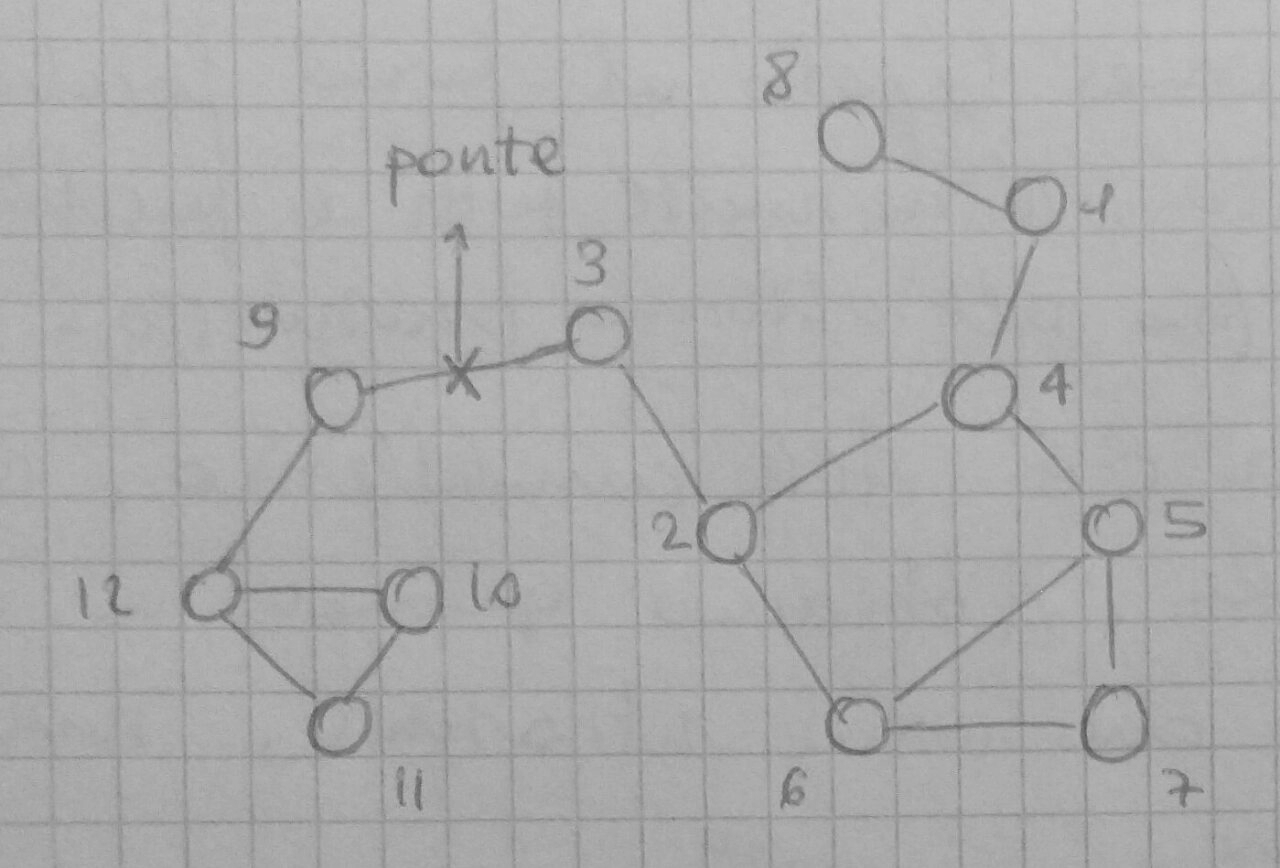
\includegraphics[width=.4\textwidth]{res/ponti-grafo.jpg} \hfill
\end{center}
Vogliamo elaborare un algoritmo che ci fornisca la lista dei ponti in un grafo.
Sappiamo che gli archi da controllare solo quelli che fanno parte dell'albero derivato dalla visita del grafo.
\begin{center}
    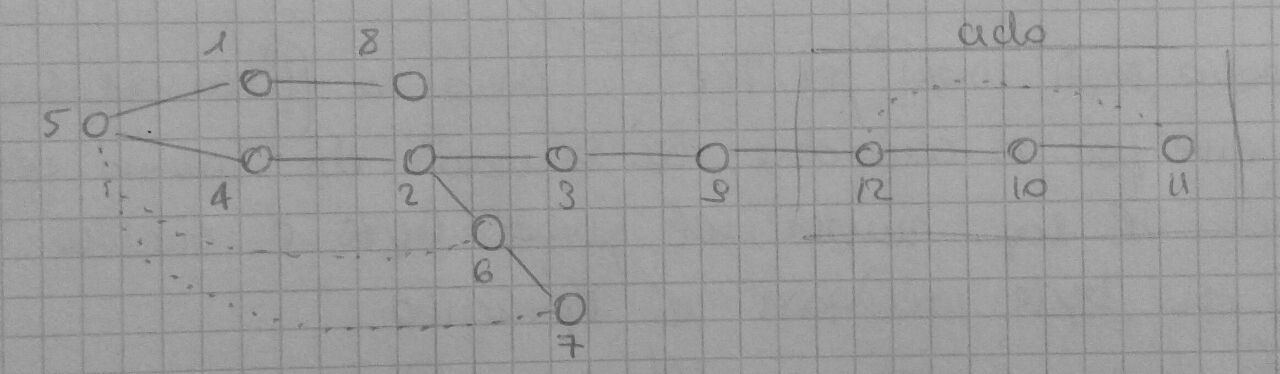
\includegraphics[width=.6\textwidth]{res/ponti-albero.jpg} \hfill
\end{center}
Tutti gli archi che non appartengono all'albero e che però erano nel grafo necessariamente non potranno essere ponti, ma saranno archi \textit{all'indietro}, \textit{in avanti} o \textit{cross}. \\
Per essere ponte, un arco deve essere arco nell'albero e non deve essere coinvolto in alcun ciclo (formato che tramite gli archi non facenti parte dell'albero). \\
Esclusi quelli, tutti i rimanenti sono ponti.
\begin{lstlisting}
# si riutilizzano i vettori Tempo, Padri, l'intero tempo
# per indicare l'ordine di visita di ciascun nodo.
DFS(u)
    tempo++
    T[u] = tempo
	vis[u] = 1 
	for y in adj(u) do
		if vis[y] = 0 then
			P[y] = u
			a = DFS(y)
			if a > T[u] then Ponti = Ponti U {y,u}
			back = min{a, back}
		else if y != P[u] then
		    back = min{T[y], back}
	return back
\end{lstlisting}
La complessità dell'algoritmo è di $O(m+n)$.

\section{Punti d'Articolazione}
I \textit{Punti d'Articolazione} sono nodi la cui rimozione sconnette il grafo. \\
In un grafo di \textit{n} nodi, questo può avere al più $n-2$ punti di articolazione. Nel caso di una catena, per esempio, . \\
Possiamo avere due tipi di alberi:
\begin{itemize}
    \item albero ad una foglia - la catena -, in cui tutti i nodi sono sicuramente punti di articolazione, esclusi il primo e l'ultimo;
    \item albero ad almeno due foglie, in cui le foglie non sono sicuramente punti articolazione.
\end{itemize}
L'algoritmo che invidivdua i punti di articolazione è molto simile a quello elaborato per individuare i ponti:
\begin{lstlisting}
# si riutilizzano i vettori Tempo, Padri, l'intero tempo
# per indicare l'ordine di visita di ciascun nodo.
DFS(u)
    tempo++
    T[u] = tempo
	vis[u] = 1 
	for y in adj(u) do
		if vis[y] = 0 then
			P[y] = u
			a = DFS(y)
			if a >= T[u] then Punti = Punti U {y}
			back = min{a, back}
		else if y != P[u] then
		    back = min{T[y], back}
    if T[u] = 1 and P[u] = 0 then
        Punti = Punti U {u}
    return back
\end{lstlisting}

\section{Sort Topologico}
Il \textit{sort topologico} rappresenta una tipologia di ordinamento lineare di grafi diretti. Nel nostro caso, desideriamo che tutti gli archi vadano solo da sinistra verso destra. \\
Non è possibile applicare questo ordinamento su tutti i grafi: infatti, l'unico caso in cui non è possibile è quello dei cicli. \\
Se è possibile applicarlo, ve ne possono essere al più $n!$ disposizioni valide diverse. \\
Un esempio banale di costruzione di un algoritmo di sorting di questo tipo è quello che seleziona per primi tutti i nodi senza archi entranti, rimuovendoli dal grafo. Se non si tratta di un ciclo, a man mano che vengono rimossi i nodi, se ne formano di nuovi senza archi entranti selezionabili, fino ad arrivare a raggiungere la situazione in cui il grafo è vuoto. \\
Prendendo come riferimento il seguente grafo:
\begin{center}
    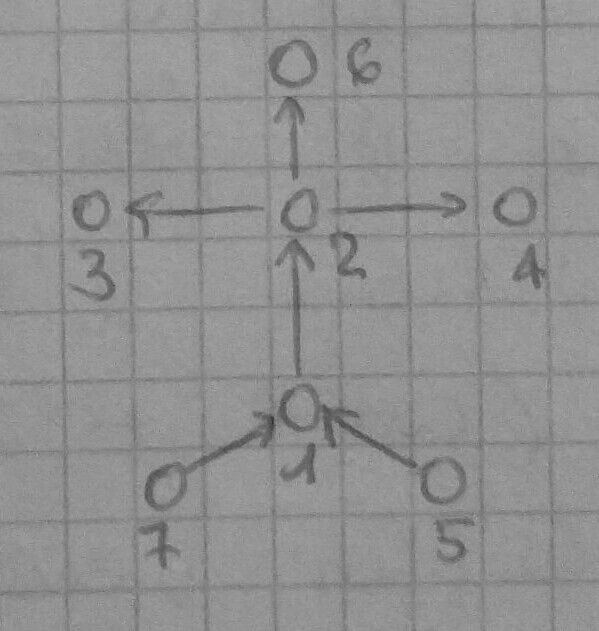
\includegraphics[width=.2\textwidth]{res/sort-topologico.jpg} \hfill
\end{center}
Un possibile output dell'algoritmo potrebbe essere la sequenza: \textit{7,5,1,2,3,6,4}.\\
Di questi, gli unici il cui ordine è fisso e non può variare senza scontrarsi con la struttura del grafo sono i due numeri \textit{1} e \textit{2}, mentre per gli altri, l'ordine è arbitrario. \\
Poiché $|\{7,5\}|=2$ e $|\{3,6,4\}|=3$, e $2!\times 3! = 2\times 1\times 3\times 2\times 1 = 12$, il numero di combinazioni possibili di sequenze che rappresentino l'ordinamento topologico del grafo è \textit{12}. \\
Avere un algoritmo che stampi \textit{tutte} i possibili ordinamenti non solo costerebbe $O((n^2)^c)$, ma il suo output sarebbe totalmente ingestibile. \\
Scriviamo quindi un algoritmo che individui \textit{uno dei} sort topologici possibili per il grafo in input:
\begin{lstlisting}
# utilizziamo una lista Sort inizialmente vuota
for i=1 to n
    if vis[i] = 0 then
        DFS[i]

DFS(u)
    vis[u] = 1
    for y in adj(u) do
        if vis[y] = 0 then DFS(y)
    aggiungi u in testa a Sort
\end{lstlisting}
Questo algoritmo costa $O(n+m)+O(n+m)$.

\section{Connessioni forti}
Si parla di \textit{grafo connesso} solo nel caso di grafi non diretti. Se il grafo è diretto occorre introdurre il concetto di \textbf{connessione forte}. \\
In un grafo, una \textbf{componente connessa} è un insieme non aumentabile di nodi raggiungibili reciprocamente a coppie. \\
Volendo definire un vettore che assegna ad ogni nodo un'etichetta diversa a seconda della sua componente, su un grafo non diretto questo vettore costa $ O(n) $ - il tempo di una visita via DFS.
Su un grafo diretto, applicare l'algoritmo sopra definito sarebbe scorretto; la direzione degli archi causa anche nei grafi diretti più semplici un livello di complessità $ O(n^2) $.


\subsection{Componenti fortemente connesse}
Il concetto di \textit{componenti fortemente connesse} - come accennato, relativo solo ai \textit{grafi diretti} - è decisamente divserso da quello delle \textit{componenti connesse} - relativo, invece, soltanto ai \textit{grafi indiretti}. \\
Si sa che per conoscere le componenti connesse, dato un grafo indiretto, occorre $ O(m+n)$. \\
Dato un grafo diretto, invece, occorre definire alcuni dati aggiuntivi:
\begin{itemize}
    \item Insieme \textit{A}: l'insieme dei nodi raggiungibili da \textit{u}, che \textit{contiene} la componente fortemente connessa (per conoscerlo, il costo è pari a quello di una visita in profondità tradizionale: $O(m+n)$);
    \item Grafo trasposto $G^T$\footnote{Dato un grafo diretto, che connette direttamente un nodo \textit{a} ad un nodo \textit{b}, si dice \textit{grafo trasposto} quello che contiene gli stessi nodi del grafo sul quale è applicata la trasposizione e i cui archi hanno inversione inversa: legherà il nodo \textit{b} al nodo \textit{a}.}: ancora, la costruzione del grafo trasposto, avrà costo pari alla visita del grafo stesso: $O(m+n)$;
    \item Insieme \textit{B}: l'insieme dei nodi che raggiungono \textit{u}, il cui costo è - ancora una volta - pari a quello di una visita \textit{del grafo trasposto}: $O(m+n)$.
\end{itemize}
Date queste informazioni, sappiamo che individuare la componente connessa relativa ad un nodo \textit{u} significherà applicare l'insersezione dei due insiemi \textit{A} e \textit{B}: $A\cap B$.
In definitiva, il costo totale sarà pari a: \\
\begin{center}
    $ O(m+n) + O(m+n) + O(m+n) = 3\times O(m+n) = O(m+n) $
\end{center}
\paragraph{NB:}
L'ultima uguaglianza è accettabile soltanto perché è nostro interesse definire l'andamento asintotico associato alla funzione. \\
\textit{A} e \textit{B} sono - come al solito - considerati dei vettori, i quali contengono \textit{1} in corrispondenza dei nodi visitati, \textit{0} altrimenti; il vettore risultante sarà \textit{CFC}, vettore contenente i risultati in \textit{AND logico} dei nodi corrispondenti in \textit{A} e \textit{B}, perché, come già detto: $ CDC = A\cap B $. \\
Dunque un grafo diretto è fortemente connesso se \textit{CFC} contiene solo \textit{1}. \\
\newpage
Per individuare tutte le componenti connesse del grafo, teoricamente, dovrei riapplicare questa procedura su tutti i nodi del grafo: $ O(n)O(m+n) $.
Per questa ragione, è stato elaborato l'algoritmo di \textit{Tarjan}. \\
Il seguente schema esplicita un esempio di applicazione dell'algoritmo:
\begin{center}
    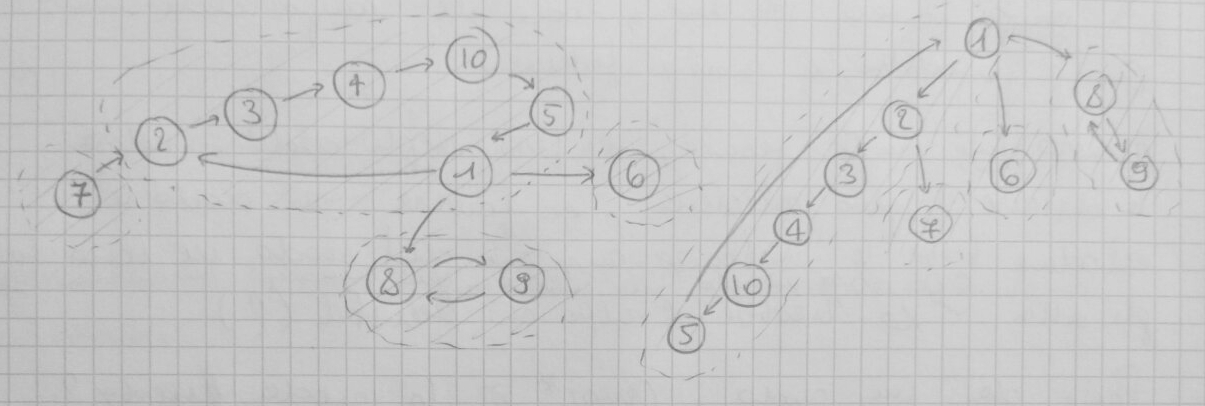
\includegraphics[width=.9\textwidth]{res/tarjan-grafo-albero.jpg} \hfill
\end{center}
Nell'albero risultante della visita, le componenti fortemente connesse rappresentano dei sottoalberi, dei \textit{grappoli}. \\
Occorre a questo punto definire il concetto di \textit{c-radice} (o \textit{c-root}): nodo che stabilisce la nascita di un sottoalbero che è componente fortemente connessa (nell'esempio proposto sopra, sono \textit{c-radici}: \textit{1}, \textit{7}, \textit{6} e \textit{8}).
Un nodo scopre di essere \textit{c-radice} durante la risalita dalla ricorsione nella visita del grafo. \\
Quindi, nell'algoritmo di \textit{Tarjan}, ogni nodo visitato a partire dalla radice, viene inserito in uno \textit{stack}; quando ritorno - per ricorsione - alla radice stessa, svuoto tutto lo \textit{stack}, che contiene i nodi che ormai sappiamo essere parte di una componente fortemente connessa. \\
Il costo totale è pari a quello della visita sommato all'analisi dello \textit{stack} (che - per deduzione -  sappiamo essere pari a $ O(n) $): $ O(m+n)O(n) $. \\
Inoltre, sicuramente, in un sottoalbero, un nodo non può essere \textit{c-radice} se un suo antenato è raggiunto da un arco \textit{back}. Ancora, l'arco \textit{cross} suggerisce un nuovo \textit{c-root} soltanto se punta ad un nodo che è già nello \textit{stack} attualmente in lavorazione.

\section{Grafo pesato}
Si definisce \textit{grafo pesato} un grafo i cui archi hanno un \textit{peso}, detto \textit{valore} o \textit{costo}. \\
Nella rappresentazione a \textit{matrice}, un \textit{grafo pesato} sarà rappresentabile sostituendo gli \textit{1}, con i \textit{pesi} degli archi. Analogamente, nella rappresentazione tramite \textit{liste di adiacenza}, si utilizzeranno non più caselle da due - contenenti il nodo e il collegamento ad un altro nodo -, ma caselle da tre - contenenti anche il \textit{peso} degli archi che legano il nodo precedente a quello descritto nella casella. \\
Avendo un grafo pesato, sappiamo che il \textit{valore} degli archi indica una distanza: voglio calcolare, a partire da un nodo \textit{u}, tutte le distanze \textit{minime} dal nodo \textit{u} a tutti quelli che sono legati (anche indirettamente) a questo stesso, costruendo un \textit{albero dei cammini}. Il seguente problema è stato risolto con l'algoritmo di \textit{Dijkstra}. \\
\newpage
Sostanzialmente, si parte dal nodo \textit{u}, indicandone - ad apice - la distanza (la distanza di \textit{u} da sé stesso è pari a \textit{0}). La regola \textit{greedy}\footnote{Con \textit{greedy} si intende una tecnica algoritmica che cerca di ottenere una soluzione ottima da un punto di vista globale attraverso la scelta della soluzione più \textit{golosa} (\textit{aggressiva} o \textit{avida}) ad ogni passo locale. Nel regno degli algoritmi \textit{greedy}, esistono gli algoritmi \textit{approssimato}: risolvono problemi con complessità esponenziale, attraverso soluzioni più approssimative rispetto a quelle assolutamene provabili.} consiste nello scegliere, a partire da quest'ultimo, \textit{sempre} il nodo raggiungibile (direttamente - tramite \textit{u} stesso - o indirettamente - tramite i nodi adiacenti ai nodi già aggiunti all'albero -) con distanza minima.
\begin{center}
    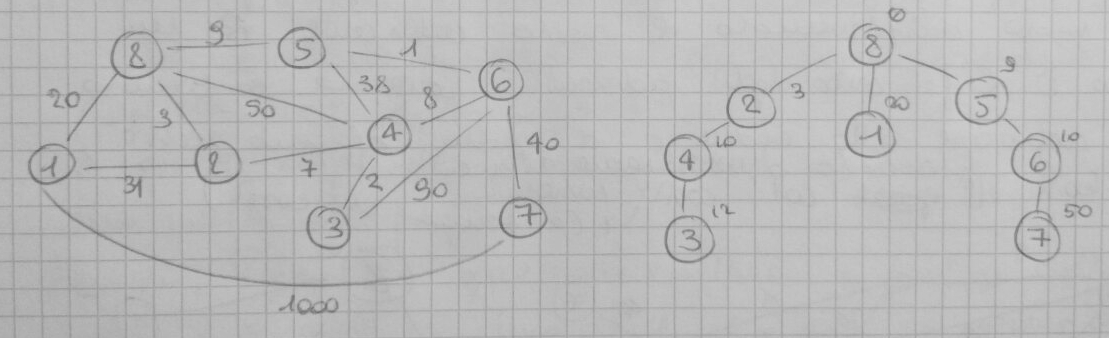
\includegraphics[width=.9\textwidth]{res/dijkstra-albero-cammini-minimi.jpg} \hfill
\end{center}
La complessità dell'algoritmo di \textit{Dijkstra} è pari a $O((m+n)\times logn)$.

\subsection{Implementazione dell'algoritmo}
\begin{algorithm}
    \caption{Ricerca di albero dei cammini minimi}\label{alg:ACM}
    \begin{algorithmic}[1]
        \Function{camminiMinimi}{}
            \State $P(u) \gets u$  \Comment{Flag di visita}
            \For { $ i \in 2 \to n $}
                \State find Arch(x,y) such that \{
                \State (P(x) != 0 \&\& P(y) = 0) such that \Comment{P: parent}
                \State (D(x) + c(x,y)) is lower value \Comment{D: distance; c: cost}
                \State \}
                \State P(y) = x
                \State D(y) = D(x) + c(x,y)
            \EndFor
            \State \textbf{return} false\Comment{}
        \EndFunction
    \end{algorithmic}
\end{algorithm}

\subsection{Dimostrazione correttezza dell'algoritmo}
Dobbiamo dimostrare che, ad ogni passo, la distanza settata è effettivamente la distanza minima dalla radice.
\begin{itemize}
    \item \textbf{CASO BASE: $ D[u] = 0 $}
        Corretto solo se nel grafo non ci sono archi con peso negativo;
    \item \textbf{PASSO INDUTTIVO: la distanza $D[i]$ è corretta, occorre verificare che lo sia anche per $D[i+1]$}
        Supponiamo che valga fino al passo i-esimo (quindi che le distanze fino a quel passo siano valide). Avremo un insieme di nodi ancora non inseriti nel nuovo albero; per ogni nodo di questo insieme ci sarà almeno un nodo collegato ad esso e già inserito nell'albero. Supponiamo che ci sia un cammino alternativo rispetto a quello 'corretto'. Ciò è assurdo: se scelgo il cammino da \textit{a} a \textit{b}, so che sicuramente costerà più di quello $D[u]$ e che \textit{b} non potrà fare altro che peggiorare la situazione, dovendo passare \textit{x} altri nodi prima di raggiungere \textit{y} (senza pesi negativi).
\end{itemize}

\subsection{Complessità dell'algoritmo}
Banalmente, si potrebbe dire che:
\begin{itemize}
    \item a causa del ciclo \textit{for}, avremo sicuramente una complessità di $O(n)$;
    \item a causa delle operazioni interne al ciclo \textit{for}, invece, di $O(n+m)$ (dove \textit{n} è il numero di operazioni eseguite dalla ricerca dell'arco, e \textit{m} per le altre).
\end{itemize}
Seguendo questo ragionamento, la complessità sarebbe pari a:
\begin{center}
    $ O(n)\times O(n+m) = O(n^2 + n\times m) $
\end{center}
Analizzando però con più precisione, consideriamo che per ogni iterazione nel ciclo \textit{for}, le verifiche da eseguire diminuiscono, perché i nodi già inseriti nei vettori, non vanno più considerati. Inoltre, poiché per trovare il minimo in un \textit{heap} occorre $\log(n)$, arriviamo a ridurre la complessità complessiva, fino a raggiungere: $O((m+n)\times \log(n))$ .

\section{Trasformazione da grafi pesati a standard}
Trasformare grafi pesati in grafi standard può risultare utile in alcuni casi, ma in linea di massima presenta alcune complicazioni nell'analisi del grafo costruito:
\begin{itemize}
    \item il numero i nodi aumenta del peso totale degli archi nel grafo originario, al quale viene sottratto il numero di archi stesso;
    \item il numero di archi diventerà pari alla somma dei pesi di tutti gli archi del grafo originario.
\end{itemize}
\newpage

\section{Albero di copertura}
L'introduzione dell'\textit{albero di copertura} deriva dalla necessità di ridurre un grafo mantenendolo connesso e con archi di costo minimo. Sostanzialmente, mentre con \textit{Dijkstra} si teneva conto dei percorsi attraversati per avere una visione oggettiva del percorso più corto selezionabile, nell'individuazione dell'arco utile alla costruzione di un albero di copertura, si seleziona \textit{sempre} l'arco con costo minore rispetto al nodo preso in considerazione nell'attraversamento del grafo.
Con l'algoritmo di \textit{Dijkstra} otteniamo un albero che connette tutto il grafo ma \textit{non} è l'albero di copertura minimo. \\

Può accadere che un albero di copertura coincida con l'albero dei cammini minimi (derivante dall'applicazione dell'algoritmo di \textit{Dijkstra}): \\
\begin{center}
	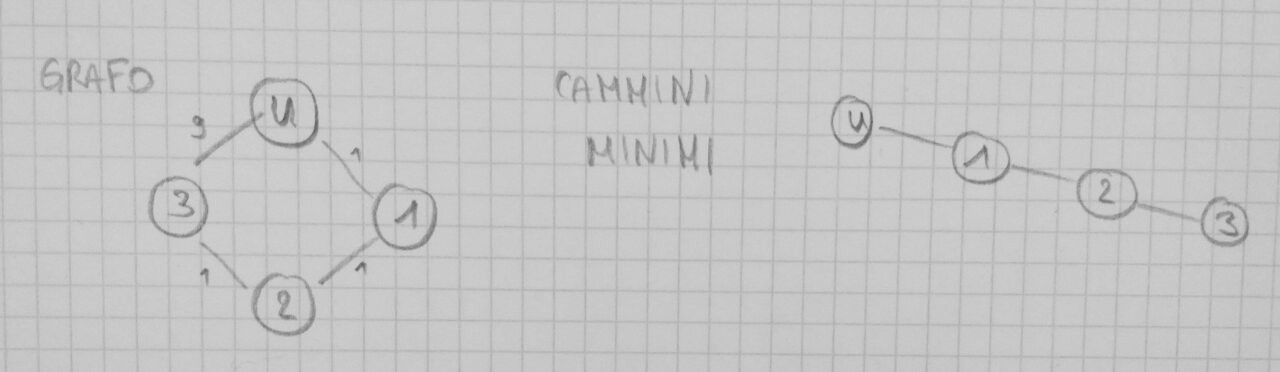
\includegraphics[width=.75\textwidth]{res/copertura-caso1.jpg} \hfill
\end{center}

Ma non è possibile assolutizzare, perché in alcuni casi questo non accade: \\
\begin{center}
	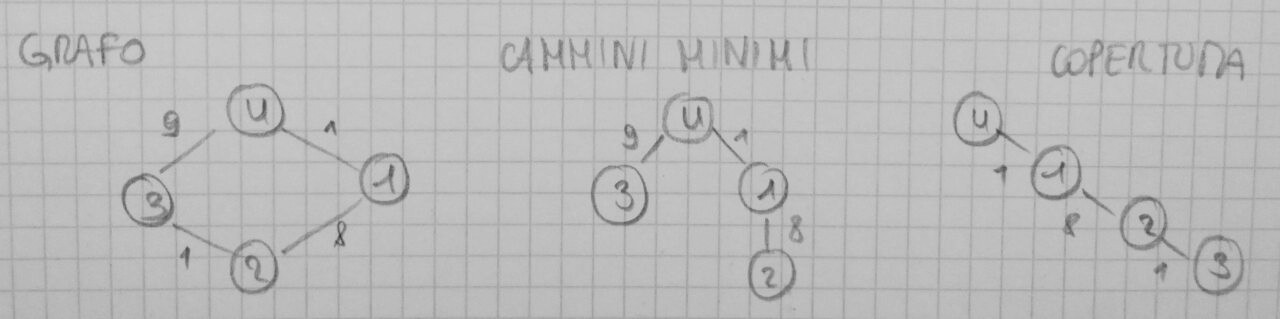
\includegraphics[width=.75\textwidth]{res/copertura-caso2.jpg} \hfill
\end{center}

Quindi, con l'algoritmo di \textit{Dijkstra} non possiamo determinare l'albero di copertura minimo. Per individuarlo, occorre utilizzare un algoritmo \textit{greedy} simile a quello di \textit{Dijkstra} ma cambiando la regola di selezione degli archi ad ogni passo. Ignorando il costo degli archi precedenti, ad ogni passo scegliamo l'arco di costo minore dal nodo in cui ci si trova al nodo che si vuole connettere.

\subsection{Analisi e costi}
Al momento, si sa che vi sono diversi costi di visita in base al tipo di struttura adoperato:
\begin{itemize}
	\item $O(n\times m)$ : tramite liste di adiacenza;
	\item $O(n^2)$ : tramite vettore;
	\item $O((n+m)\times \log(n))$ : tramite \textit{heap};
	\item $O(m+n\times \log(n))$ : tramite \textit{heap} di \textit{Fibonacci}.
\end{itemize}
Uno stesso grafo può avere più alberi di costo minimo differenti.

\subsubsection{Dimostrazione validità}
Si vuole dimostrare che se un grafo è connesso abbiamo almeno un albero di copertura.
Chiamiamo $T_{o\ldots n}$ gli archi presenti nell'albero parziale nato dalla visita fino al passo \textit{n}, e dimostriamo :
\begin{center}
	$\forall i : T_{i} \subseteq T^*$ \\
	dove $T^*$ è l'albero di copertura ottimale
\end{center}
\paragraph{Passo base}
$T_{0} = \phi \Rightarrow T_{0} \subseteq T^* \Rightarrow$ il passo base è verificato.
\paragraph{Passo induttivo}
$T_{i} \subseteq T^*$ per ipotesti induttiva. Ma per $T_{i+1}$? \\
Sicuramente sappiamo che $T_{i+1} = T_{i} \cup \{e\}$, dove \textit{e} è l'arco di costo minimo a partire nal nodo attualmente selezionato. Ma $T_{i} \cup \{e\} \subseteq T^*$? Possono accadere due casi: o \textit{e} è presente, o non lo è. \\
Se \textit{e} è presente in $T^*$ abbiamo dimostrato la correttezza dell'ipotesi. Se invece non lo è, allora $T^*$ non è la soluzione ottimale che cerchiamo, ma potrebbe esistere un'altra soluzione ottimale che contiene anche \textit{e}. \\
Quindi, $T_{i+1} \cup \{e\} \subseteq T^* \cup \{e\} - \{e^1\}$: per mantenere il contenimento vero, bisogna togliere un arco $e^1$ che non è contenuto in $T^*$.
Questo ragionamento nasconde il fatto che il grafo nasconde archi diversi con pari costo, motivo per cui siamo abilitati a non dare eccessiva importanza alla rimozione dell'arco $e^1$.

\subsection{Algoritmo di Kruskal}
Tramite l'algoritmo di \textit{Kruskal}, si individua un albero di copertura attraverso un sistema diverso. Partendo da un grafo, si selezionano sequenzialmente tutti gli archi - da quello con costo minimo a quello con costo massimo: se l'arco stabilisce un ciclo con gli archi precedentemente selezionati, viene scartato, altrimenti preso. \\
Tale algoritmo ha costo $O(m\times \log(m))$ (asintoticamente pari a $O(m\times \log(n))$; quantitativamente parlando, invece, $(m\times \log(m)) \geq (m\times \log(n))$).

\begin{algorithm}
	\caption{Ricerca di albero di copertura}\label{alg:AC}
	\begin{algorithmic}[1]
		\Function{alberoCopertura}{}
		\State $T \gets \phi$  \Comment{Inizializzazione albero}
		\While {$ |E| \neq \phi $}
		\State estrai arco \textit{e} di costo minimo da \textit{E}
		\If {\textit{e} non forma ciclo con \textit{T}}
			\State $T \gets T \cup \{e\}$
		\EndIf
		\EndWhile
		\State \textbf{return} \textit{T}
		\EndFunction
	\end{algorithmic}
\end{algorithm}

Estrarre l'arco di costo minimo costa $O(n)$ se non ottimizzo e uso una lista. Se invece ordiniamo per estrarre il minimo dalla testa, paghiamo $O(1)$. Per ordinare spendiamo - una sola volta - $O(m\times \log(m))$. Controllare se l'arco stabilisce un ciclo con gli archi già visitati significa visitare \textit{T} in $O(n)$. Il \textit{while} costa, invece, $O(m)$. \\
Dunque il \textit{while} viene eseguito esattamente \textit{n} volte, ovvero il numero degli archi, e non si può far niente per migliorarlo. L'\textit{if}, senza ottimizzazioni impiega $O(m\times n)$. \\
Vogliamo fare in modo di trasformarlo in $\log(n)$: l'idea è quella di usare una struttura dati, \textit{onion n file}. Non voglio arrivare al migliore modo di implementare questa struttura, ma l'obiettivo è quello di raggiungere $m \log(n)$ (meno non avrebbe granché senso asintoticamente parlando, a causa del costo dell'ordinamento, che appunto è questo). \\
Dato un \textit{heap} vogliamo sapere se un arco crea un ciclo in un albero. Questa operazione sarebbe fatta in modo efficiente se c'è un coefficiente per scoprire, dati due componenti,m se sono nella stessa componente connessa. Se è così, non dovrò aggiungerlo, sì, altrimenti. Sostanzialmente, occorre una struttura dati, per \textit{strutturare i dati} (i nodi, nello specifico), in modo tale da poter in modo efficiente rispondere alla domanda: \textit{due nodi sono nella stessa componente?} In più deve essere facilmente aggiornabile, perché si vuole che si fondano due componenti - precedentemente sconnesse - in una connessa. \\
Avrò quindi bisogno di due operazioni:
\begin{itemize}
	\item un metodo \textit{find(x)} che, dato un nodo \textit{x}, mi restituisca la componente di quel nodo;
	\item un metodo \textit{union(a,b)} che, date due componenti \textit{a} e \textit{b}, le unisca.
\end{itemize}

\begin{algorithm}
	\caption{Ricerca di albero di copertura con \textit{find} e \textit{union}}\label{alg:AC2}
	\begin{algorithmic}[1]
		\Function{alberoCopertura}{}
			\State $T \gets \phi$  \Comment{Inizializzazione albero}
			\State ordina \textit{E} in maniera crescente
			\While {$ |E| \neq \phi $}
				\State estrai arco \textit{e} di costo minimo da \textit{E}
				\State $a \gets find(x)$
				\State $b \gets find(y)$
				\If { $a \neq b$}
					\State $T \gets T \cup \{e\}$
					\State $union(a,b)$
				\EndIf
			\EndWhile
			\State \textbf{return} \textit{T}
		\EndFunction
	\end{algorithmic}
\end{algorithm}
Inizialmente, ogni volta che viene eseguita la \textit{union(a,b)} diminuirà di 1 il numero di componenti connesse, per cui l'algoritmo verrà eseguito \textit{n} volte e il costo dell'altra parte sarà di $n\times O(union)$. Questo sarebbe il costo dell'algoritmo, perché all'inizio $O(m \times \log(n))$, poi $m\times O(find)$ e $n\times O(union)$. \\
Con questa implementazione \textit{find} costerà $O(1)$ e \textit{union} $O(n)$, aumenterà perché la \textit{union} costerà totalmente $O(n^2)$. A noi serve un'implementazione più avanzata, perché questa fa molto bene il \textit{find}, ma non l'\textit{union}. \\
A noi occorre che le \textit{union} siano eseguite in maniera efficiente e che le \textit{find} costino $O(\log(n))$, in modo che le \textit{union} impieghino \textit{n}. \\
Il modo migliore è pensare una regola per cui la \textit{union} che unisce due componenti con nome diversono, nella risultante mantengono quello della più piccola: $min(a,b) = a$. In questo modo, la componente \textit{b} prenderà nome \textit{a}. Sembra che così costi $O(1)$: vado nel vettore, e quando devo unire le due componenti vado a vedere in \textit{a} cosa c'è, poi in \textit{b}, prendo il più piccolo e lo metto nel massimo. \\
Dopo aver cambiato 10 nodi, dovrò unirla con una componente che ha nome più piccolo, non solo deve cambiare il nome di quell'elemento, ma anche di tutti i 10 nodi con cui questo era connesso. Occorre quindi scorrere tutto il vettore ed ogni volta che si incontra il vecchio nome, sostituirlo con il nuovo: funziona ed ha costo $O(n)$.

\subsubsection{Metodo più efficiente}
Costruisco un \textit{tabloid}: ho una lista a puntatori, ognuno punta a sé stesso. Nel momento in cui inserisco nel grafo un arco \textit{(a,b)}, queste due liste a puntatori \textit{a} e \textit{b} le unisco in una lista unica: quale delle due? Non è granché importante, possiamo utilizzare il meccanismo del rapporto \textit{padre-figlio} tra i nodi. Ma in questo caso non posso farlo più in $O(1)$, perché devo salire dalle varie componenti, per scoprire se la componente in cui si trova un determinato tramite il vettore dei padri mi muovo all'interno della lista finché non arrivo alla radice. La radice sarà quella che dà il nome alla componente. Ad esempio, \textit{a} punta a sé stesso, e \textit{b} punterà a \textit{a}, perciò \textit{b} sarà in \textit{a}. \\
Quando devà fare la \textit{union} trasformo semplicemente gli indici, faccio un \textit{find} sul primo e secondo elemento, poi quello che faccio è che la componente più grande diventa figlia di quella più piccola: ad esempio, se unisco $a=(2,3)$ e $b=(4,5)$, accade che l'unica cosa che dovrò fare è far puntare 4 a 2. \\
Questo vuol dire che dopo che ho fatto le due \textit{find}, la \textit{union} richiede soltanto di cambiare il nome ad una delle due, di farla puntare a quella più piccola. Questa operazione costerà soltanto $O(1)$. La \textit{find}, dato un nodo, per scoprire la componente, richiede che io risalga fino a raggiungere la radice, un nodo in cui il padre è sé stesso. Costa $O(n)$, ma noi volevamo costasse $O(\log(n))$. Ma con questo meccanismo gli albero possono diventare molto lunghi, perché per ogni componente unita creo un nuovo \textit{alberello} a sé stante. Quello che occorre fare è scegliere di far puntare quello più piccolo a quello più grande: usando questa tecnica, l'albero risultante rimarrà bilanciato. \\
Vogliamo dimostrare che usando questo artificio, quello che ha l'altezza minore diventa padre e quello con altezza maggiore diventa figlio e allora le catene non potranno essere più lunghe di $\log(n)$.
\paragraph{Dimostrazione}
Dimostriamo che un albero di altezza \textit{i} avrà al massimo $2^i$ nodi. \\
Poiché in un albero al pià che ne possono essere \textit{n}, quindi $2^i \le n$. Allora $i \le \log(n)$. Di conseguenza, qualsiasi altezza non potrà superare $\log(n)$. \\
Se l'altezza è pari a 0 - non avendo fatto \textit{union}, allora avremo $2^0$ nodi, quindi è vero. Vale lo stesso anche con una \textit{union} in più. Con una \textit{union} in più, un albero che aveva una certa altezza può aumentare, ma poiché il più piccolo lo rendo figlio se il più piccolo non aveva altezza \textit{i}, cambia l'altezza del nuovo albero solo quando i due alberi hanno la stessa altezza: uno dei due aumenta di uno. L'altezza quindi diventerà $i+1$, ma per ipotesi induttiva, poiché aveva altezza \textit{i}, aveva almeno $2^i$ nodi, e la somma di questo è almeno $2^i + 2^i = 2^(i+1)$. Il meno profondo deve diventare figlio del più profondo, ed intuitivamente questo significa che le altezze non crescono, ameno che siano uguali in cui aumenterà semplicemente di \textit{1} l'altezza. \\
Usiamo quindi il vettore dei padri ed ogni volta che devi unire, questa volta avrai una foresta (tanti alberi diversi) e quando vuoi conoscere la componente risali a quel nodo e raggiungi la radice (quella è la componente). Questa risalita non costerà mai più di $\log(n)$. Cambiare il puntatore costerà solo $O(1)$.